\section{Creating an ICE Item} 

This tutorial will teach you how to
create your own ICE Items via the built-in tools within ICE.  To demonstrate
these tools, we will walk through the development of a dashboard for the
FERN code, a fast, efficient nuclear reaction network solver. 

After creating a new ICE Item plugin project, we will demonstrate how to
provide a few lines of code to create an editor for
input files for FERN. After that we will show how a small amount of code can be
used to create a job launcher that is customized to execute FERN locally. We
will also show how to launch FERN remotely.

\subsection{Creating the Plug-in Project}

\begin{figure}[h]
\centering
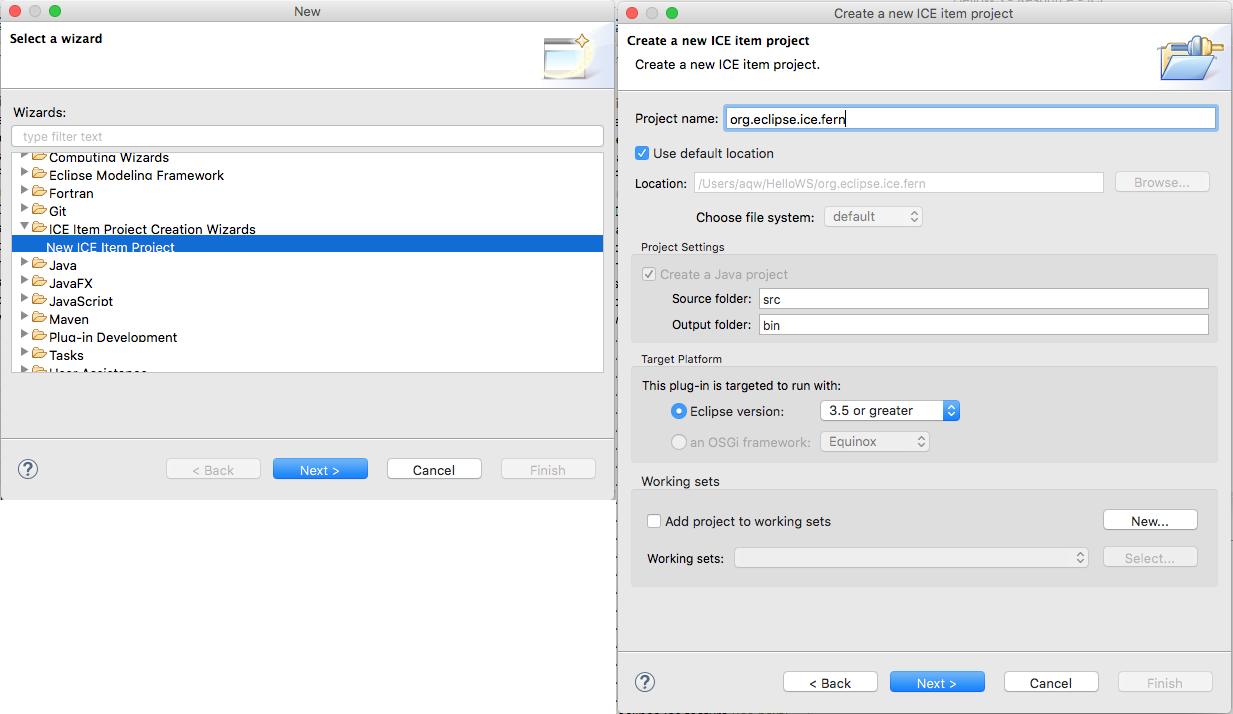
\includegraphics[width=\textwidth]{figures/comb12.png}
\label{fig:comb12}
\end{figure}

To create a new ICE Item project, navigate to \texttt{File $\rightarrow$ New
$\rightarrow$ Other}. Open the \texttt{ICE Item Creation Wizards} folder and 
select \texttt{ICE Item Creation Wizard}. You will be met with a standard new
project wizard page, in which you can name your project.  We will call ours
\texttt{org.eclipse.ice.fern}. Once you have named your project click the \texttt{Next>} button.
\begin{center} 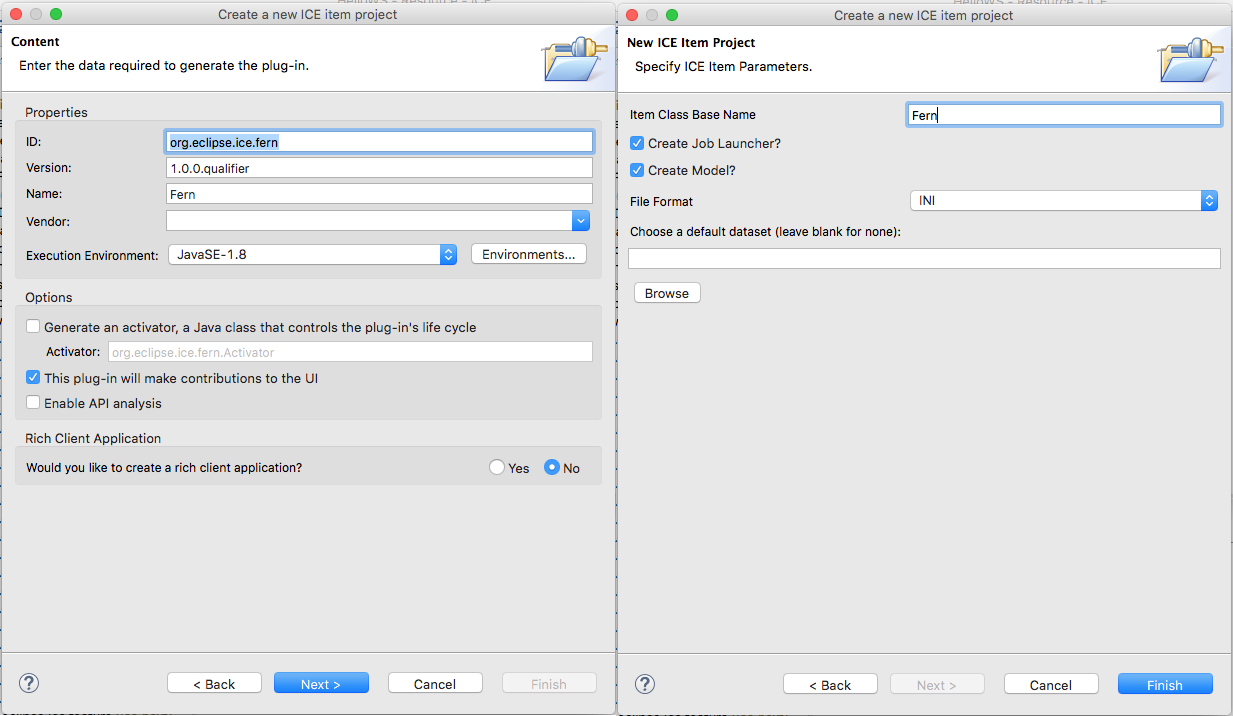
\includegraphics[width=\textwidth]{figures/comb23} \end{center}

The next dialog page enables you to customize the plugin-specific
portions of the project. For this tutorial, we will leave all the settings at
their defaults. Simply click \texttt{Next>} to move to the next page. 

On this page you need to tell the wizard what you want to use as a base
name for your item classes. We will call this one \texttt{Fern}. Then, we will
specify some information about how the item will handle input data.  FERN uses
the INI file format to specify data, so we will tell our item to use the built-in
functionality for INI files.  To do this select \texttt{INI} from the \texttt{File Format} dropdown.  

When you have entered all of the required information you can
click the \texttt{Finish} button to generate your new ICE Item plugin project.
When the project has finished generating you should be able to explore the code
that has been created.  Within the source directory there will be two packages,
each containing two Java classes:

\begin{itemize} 
    \item \texttt{org.eclipse.ice.fern.launcher} 
    \begin{itemize}
        \item \texttt{FernLauncher.java} 
        \item \texttt{FernLauncherBuilder.java}
    \end{itemize} 
    \item \texttt{org.eclipse.ice.fern.model} 
    \begin{itemize} 
        \item \texttt{FernModel.java} 
        \item \texttt{FernModelBuilder.java}
    \end{itemize} 
\end{itemize}

To add functionality to the project we need to edit
the \texttt{FernLauncher} and \texttt{FernModel} classes.

\subsection{Adding Functionality to the New Items}

\subsubsection{The Fern Model}

The \texttt{FernModel} will be responsible for creating and
validating input parameters for FERN, in the form of a new FERN input file.  In
order to make the generated code run there are several pieces of information that need to be changed.  First, we
will need to set up the basic Item identification information. This information
is set in the setupItemInfo() method. Modify the outputName to match the
following (or something of your choosing, with a .ini file extension).

\begin{lstlisting}[language=Java]
outputName = "fern_config.ini";
\end{lstlisting}

The String for the \emph{setName} method will serve as the display name
for this Item, so set it as \texttt{Fern Model}.
As for the String for \emph{setDescription}, this will also be used on the UI
for the Item, so provide some text like the following: \texttt{This Item constructs input files
for the FERN reaction network solver}. The export string will serve as the name
of the action that the user can select to write the provided data to file. Set
it to something like: \texttt{Export to INI}. You should now have a method that
looks like this:

\begin{lstlisting}[language=Java]
@Override
protected void setupItemInfo() {
	setName("Fern Model");
	setDescription("This Item constructs " +
	    "input files for the FERN reaction " +
	    "network solver"); 
	outputName = "fern_config.ini";   
	exportString = "Export to INI";
	allowedActions.add(0, exportString);
	ioFormat = "INI";
	defaultFileName = "";
}
\end{lstlisting}

The \emph{allowedActions.add()} line ensures that the export string is provided
to ICE as an allowed action, and displayed in the Item Process drop down.

With the identification information configured properly we can begin to
implement the Form for this FERN Model. This is done in the \emph{setupForm()}
method.
The generator has begun the process of implementing this method by instantiating
a Form for you to use, getting a reference to the IOService (which provides
IReader/IWriter realizations), and providing a commented out example of how to
fill out an ICE Form.

For this FERN input model, we want to add the following sections with data
entries: a network section with 
numSpecies, numReactions, numReactionGroups, massTol, fluxFrac, networkFile,
rateFile data entries, an initialConditions section with T9, startTime, endTime,
initialTimeStep, and density, and an output section with a single popFile
data entry.
To achieve this for this Item, we will need to add three
\texttt{DataComponents}, one for the network section, another for the
initialConditions section, and a final one for the outputs section. To each of
those DataComponents we will add appropriate IEntry instances for each of the data entries we have.

Add the following to your setupForm() method: 

\begin{lstlisting}[language=Java]

    // Create the network section
    DataComponent networkComp = new DataComponent();
    networkComp.setName("network");
    networkComp.setDescription("The parameters needed " +
        "to describe the nuclear " +
    	"reaction network"); 
    networkComp.setId(1);
    
    // Create the IEntries we need for this DataComponent
    StringEntry numSpecies = new StringEntry();
    numSpecies.setName("numSpecies");
    numSpecies.setDescription("The number of species to consider");
    numSpecies.setDefaultValue("16");
    
    StringEntry numReactions = new StringEntry();
    numReactions.setName("numReactions");
    numReactions.setDescription("The number of reactions to consider");
    numReactions.setDefaultValue("48");
    
    StringEntry numReactionGrps = new StringEntry();
    numReactionGrps.setName("numReactionsGroups");
    numReactionGrps.setDescription("The number of reaction " + 
    	"groups to consider"); 
    numReactionGrps.setDefaultValue("19");

    StringEntry massTol = new StringEntry();
    massTol.setName("massTol");
    massTol.setDescription("The mass tolerance to consider");
    massTol.setDefaultValue("1.0e-7");
    
    StringEntry fluxFrac = new StringEntry();
    fluxFrac.setName("fluxFrac");
    fluxFrac.setDescription("The flux fraction to consider");
    fluxFrac.setDefaultValue(".01");
    
    FileEntry networkFile = new FileEntry(".inp");
    networkFile.setProject(project);
    networkFile.setName("networkFile");
    networkFile.setDescription("The network file for this problem");
    
    FileEntry rateFile = new FileEntry(".data");
    rateFile.setProject(project);
    rateFile.setName("rateFile");
    rateFile.setDescription("The rate file for this problem");
    
    networkComp.addEntry(numSpecies);
    networkComp.addEntry(numReactions);
    networkComp.addEntry(numReactionGrps); 
    networkComp.addEntry(massTol);
    networkComp.addEntry(fluxFrac);
    networkComp.addEntry(networkFile);
    networkComp.addEntry(rateFile);
    
    // Create the initial conditions section
    DataComponent initConditionsComp = new DataComponent();
    initConditionsComp.setName("initialConditions");
    initConditionsComp.setId(2);
    initConditionsComp.setDescription("The parameters " +
    	"needed to describe the	initial " + 
    	"conditions for the problem");
    
    StringEntry t9 = new StringEntry();
    t9.setName("T9");
    t9.setDescription("The temperature in Kelvin x 10^9");
    t9.setDefaultValue("7.0");

    StringEntry startTime = new StringEntry();
    startTime.setName("startTime");
    startTime.setDescription("The start time for the simulation.");
    startTime.setDefaultValue("1.0e-20");

    StringEntry endTime = new StringEntry();
    endTime.setName("endTime");
    endTime.setDescription("The end time for the simulation");
    endTime.setDefaultValue("1.0e-8");

    StringEntry initialTimeStep = new StringEntry();
    initialTimeStep.setName("initialTimeStep");
    initialTimeStep.setDescription("The initial time step " + 
    	"for the simulation."); 
    initialTimeStep.setDefaultValue("1.2345e-22");

    StringEntry density = new StringEntry();
    density.setName("density");
    density.setDescription("The initial density.");
    density.setDefaultValue("1.0e8");
    
    initConditionsComp.addEntry(t9);
    initConditionsComp.addEntry(startTime);
    initConditionsComp.addEntry(endTime);
    initConditionsComp.addEntry(initialTimeStep);
    initConditionsComp.addEntry(density);
    
    // Create the outputs section
    DataComponent outputComp = new DataComponent();
    outputComp.setName("output");
    outputComp.setDescription("The parameters needed to output data.");
    outputComp.setId(3);
    
    StringEntry popFile = new StringEntry();
    popFile.setName("popFile");
    popFile.setDescription("The name of the output populations file");
    popFile.setDefaultValue("popFile.csv");
    
    outputComp.addEntry(popFile);
    
    // Add the components to the Form
    form.addComponent(networkComp);    
    form.addComponent(initConditionsComp);
    form.addComponent(outputComp);
    
\end{lstlisting}

Now we have a Form constructed for a typical FERN execution. 

The default generated implementation of the process method is sufficient to be
able to create new FERN INI input files. 

\subsubsection{Fern Launcher}
A FERN launcher handles the actual execution of the FERN application. The
generator creates the FernLauncher as a subclass of ICE's JobLauncher, which
provides a large array of features and functionality. As a subclass of
JobLauncher, the FernLauncher enables users to execute FERN locally or remotely.
To do so, we just need to add a small amount of
code that customizes the ICE job launching capabilities for FERN. 

The first bit of code to add to the FernLauncher specifies the name of the
actual Fern executable. In the setupItemInfo() method, set the execCommand to
the following: 
\begin{lstlisting}[language=Java]
execCommand = "${installDir}fern-exec";
\end{lstlisting}
This tells ICE that the FERN executable is called \texttt{fern-exec}, and to
set the overall execution command to it's install path plus the executable name.
The installDir flag will tell ICE to insert the user-specified executable
location (provided through the graphical form editor') into the execCommand,
with a trailing OS-specific path separator. This install directory is
specified through the Hosts Table on the editory. 

We also need to inform the JobLauncher what other files are involved in this
execution. To do that, the JobLauncher provides an addInputType() method. Add
the following to setupForm():
\begin{lstlisting}[language=Java]
addInputType("Network File", "networkFile", 
			"Network File Description", ".inp");
addInputType("Rate File", "rateFile", "
			Rate File Description", ".data");
\end{lstlisting}

And that should be it.
The generator has taken care of everything else for us.
We are now ready to launch ICE with our FERN plugin, and use the FERN Items we
have just created.
